\chapter{平面フレームの製作工程について}

平面フレームを成型するにための型は,ベニヤ板を切り抜いた木枠を用いて製作を行った.

\section{木型の設計}
型の設計は3DCADを用いて行った.平面積層用の木枠は,ベニヤ板をレーザー加工機を用いて切り抜き,制作を行った.雄型,雌型をそれぞれ設計を行った.

\begin{figure}[htbp]
  \begin{center}
    \includegraphics[width=120mm]{img/3.JPG}
    \end{center}
  \caption{フレームの3Dモデル}
 \label{fig:robot}
\end{figure}

\section{レーザー加工機でのカーボンクロスの切り出し}
カーボンクロスをレーザー加工機を用いて切り出す.レーザー加工機を使用する以前は,ハサミで切って切り出していた.しかしカーボンクロスの繊維が細かく,ささくれてしまい積層が困難だった.レーザー加工を行うことで,縁が溶着硬化することができるため積層が綺麗に行うことができる.

\begin{figure}[htbp]
  \begin{center}
    \includegraphics[width=120mm]{img/5.JPG}
    \end{center}
  \caption{切り出されるカーボンクロス}
 \label{fig:robot}
\end{figure}


\section{木型への離型剤吹付け作業}
カーボンクロスの積層には,硬化させるためのエポキシ樹脂を用いる.そのため硬化後に離型を容易にするために離型剤を用いる.平面フレーム用の木型には,枠の縁などに塗りやすいようにスプレー式を用いた.

\begin{figure}[htbp]
  \begin{center}
    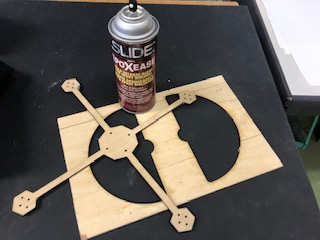
\includegraphics[width=120mm]{img/18.JPG}
    \end{center}
  \caption{離型剤の吹き付けた型}
 \label{fig:robot}
\end{figure}

\section{積層作業}
平面積層においては切り出されたカーボンクロスを枠に合わせ,1枚重ねるごとにエポキシ樹脂を塗り重ね繰り返し行う.重ねる枚数が増えてゆくにつれ塗る硬化剤の量を減らしてゆく.

\begin{figure}[htbp]
  \begin{center}
    \includegraphics[width=120mm]{img/7.JPG}
    \end{center}
  \caption{積層作業}
 \label{fig:robot}
\end{figure}

\section{仕上げ作業}
24時間以上が経過し完全に硬化したフレームは,やすり掛けバリ取りを行い完成となる.

\begin{figure}[htbp]
  \begin{center}
    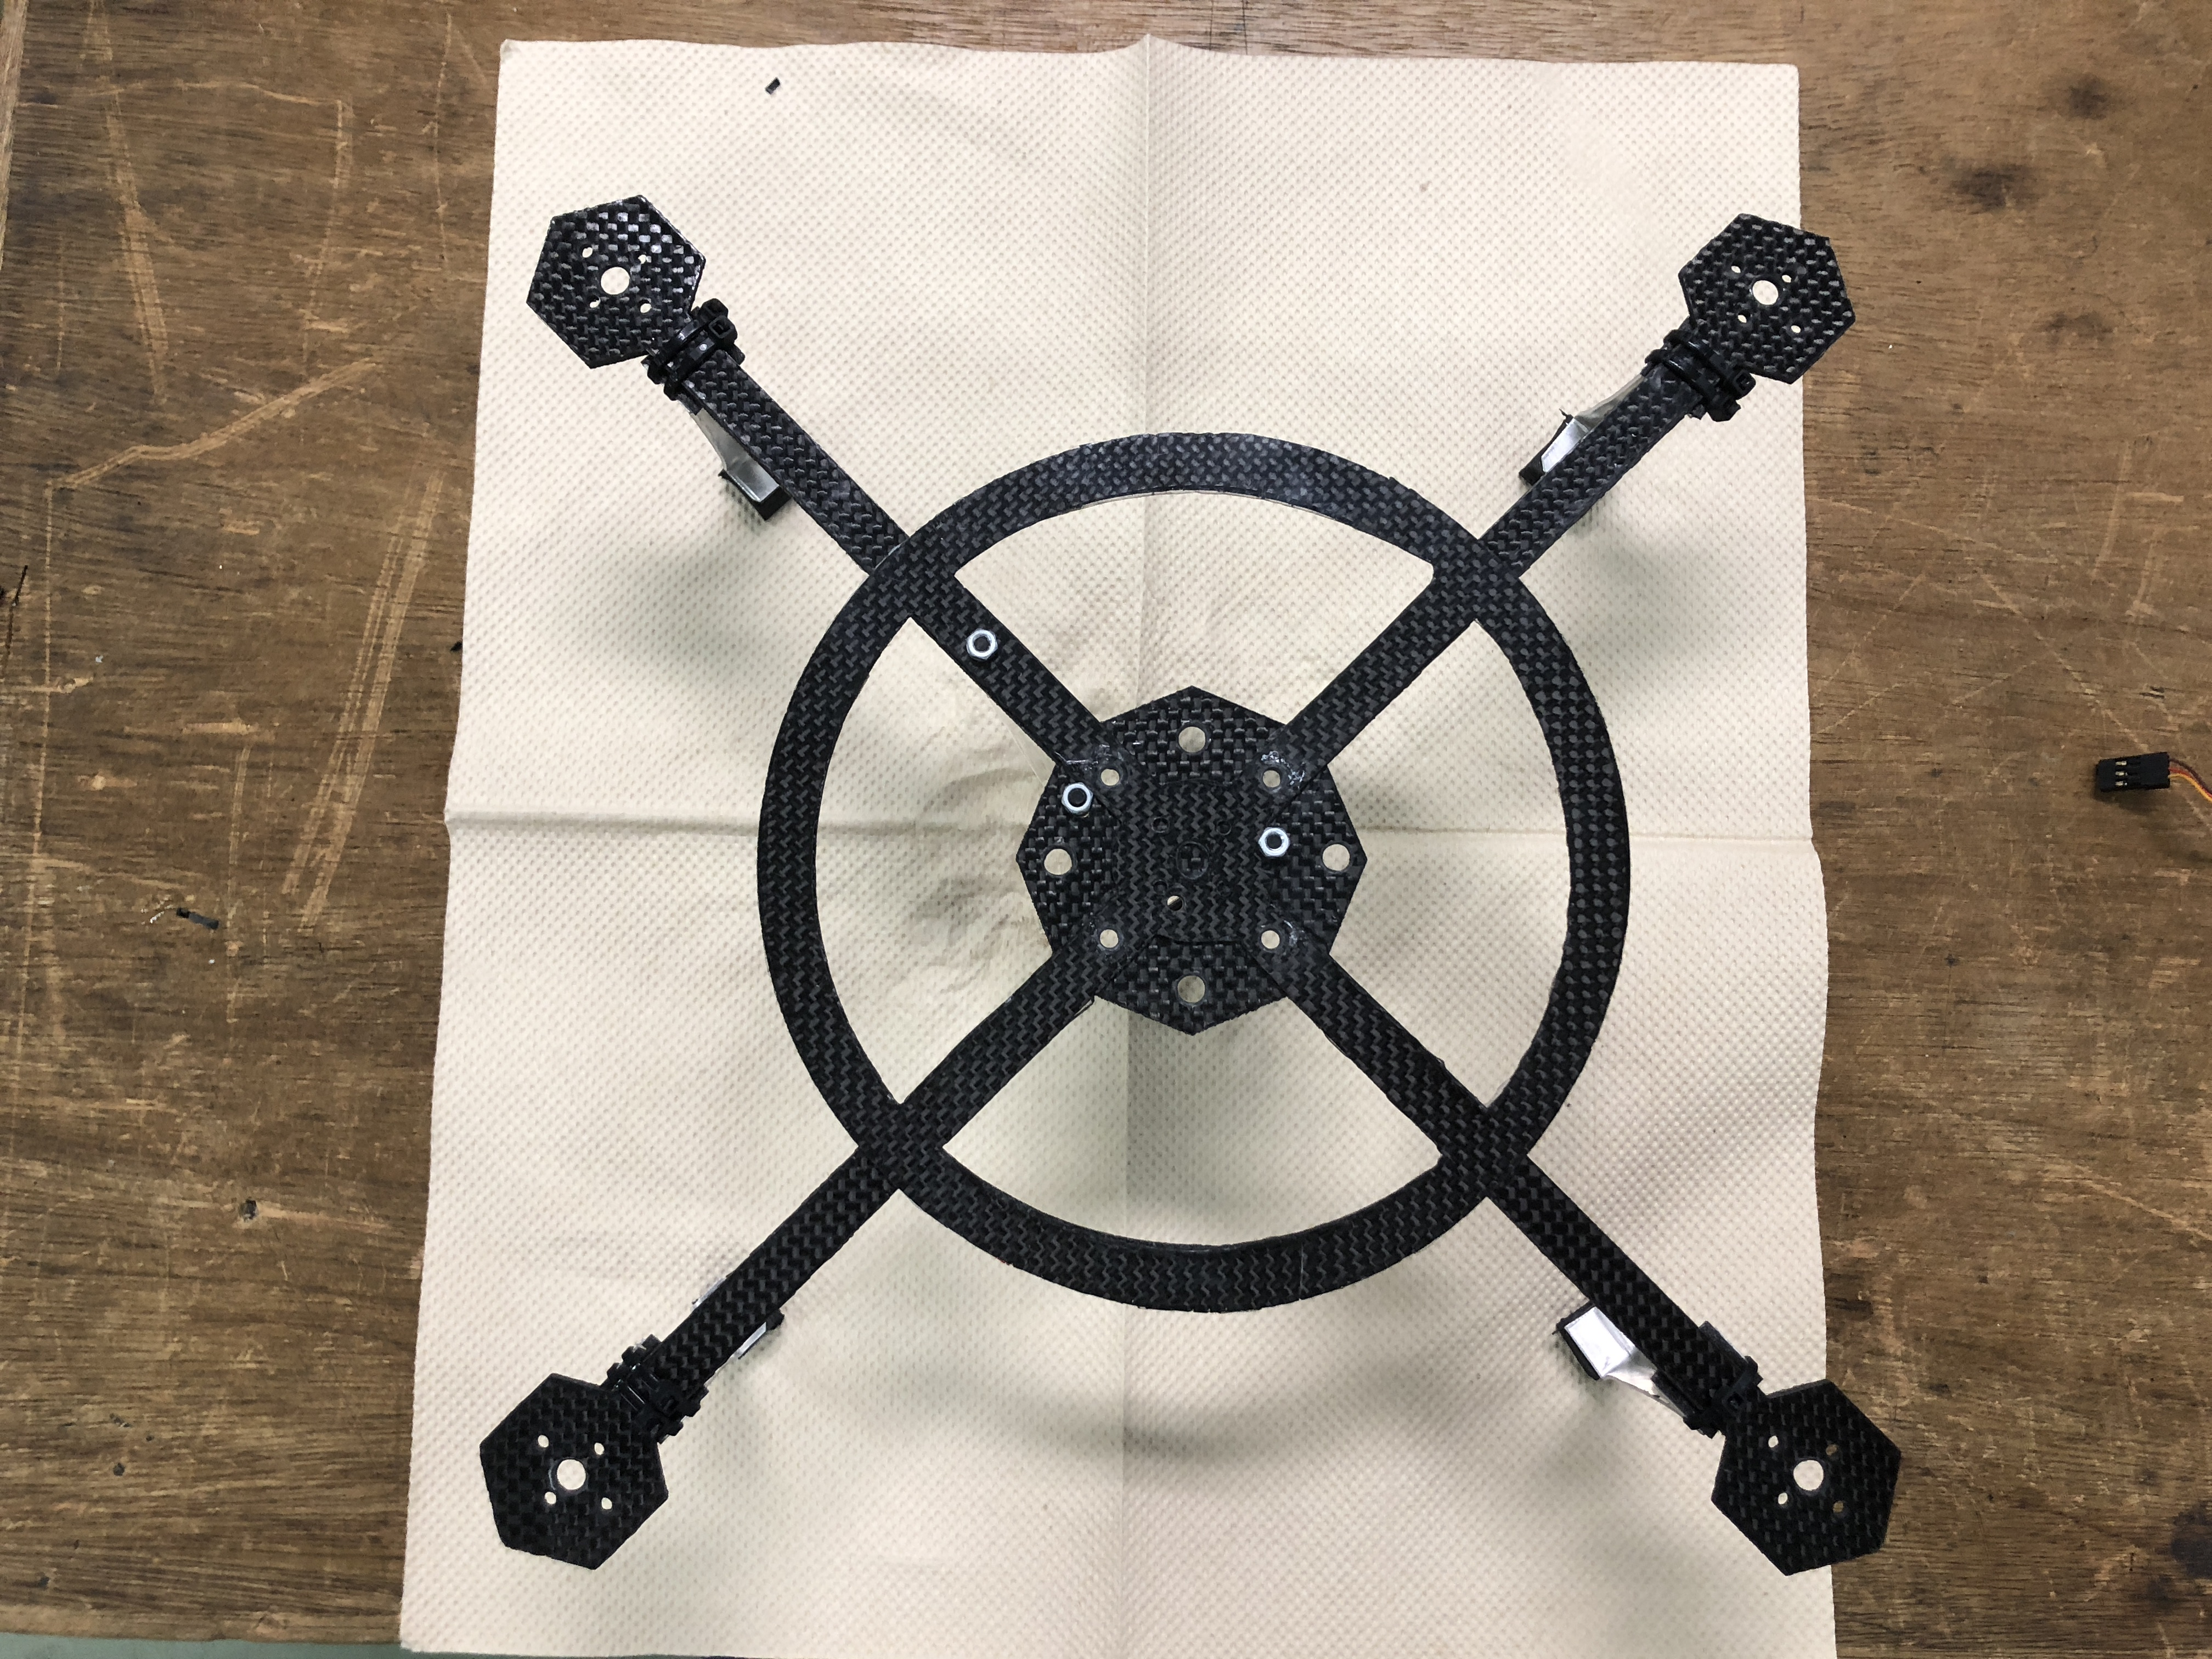
\includegraphics[width=120mm]{img/21.JPG}
    \end{center}
  \caption{完成したフレーム}
 \label{fig:robot}
\end{figure}

\section{平面フレーム製作過程においてのまとめ}
平面フレーム製作において積層硬化後,離型にエポキシ樹脂用スプレー型離型剤とポリプロピレンフィルムを用いた,どちらも容易に離型することはできたが,離型後の表面状態が異なった,スプレー型の専用のモノを使った場合,表面はつやがないマットな仕上がりとなった,しかし,散布する量にむらがあったり,量が多くなりすぎると表面に固着してしまい仕上がり面が綺麗にならないことがあった,それに対しフィルムを用いた場合は,仕上がり面は光沢となり,量による影響も全くないため表面積層においてはポリプロピレンフィルムを用いることが最適である,また平面積層において機体の足部分を,板金で湾曲させた板を用いて立体積層も行った.しかし湾曲部に角がついてしまい着陸時の衝撃ですぐに破損してしまい,平面での立体積層は困難であった.

\begin{figure}[htbp]
  \begin{center}
    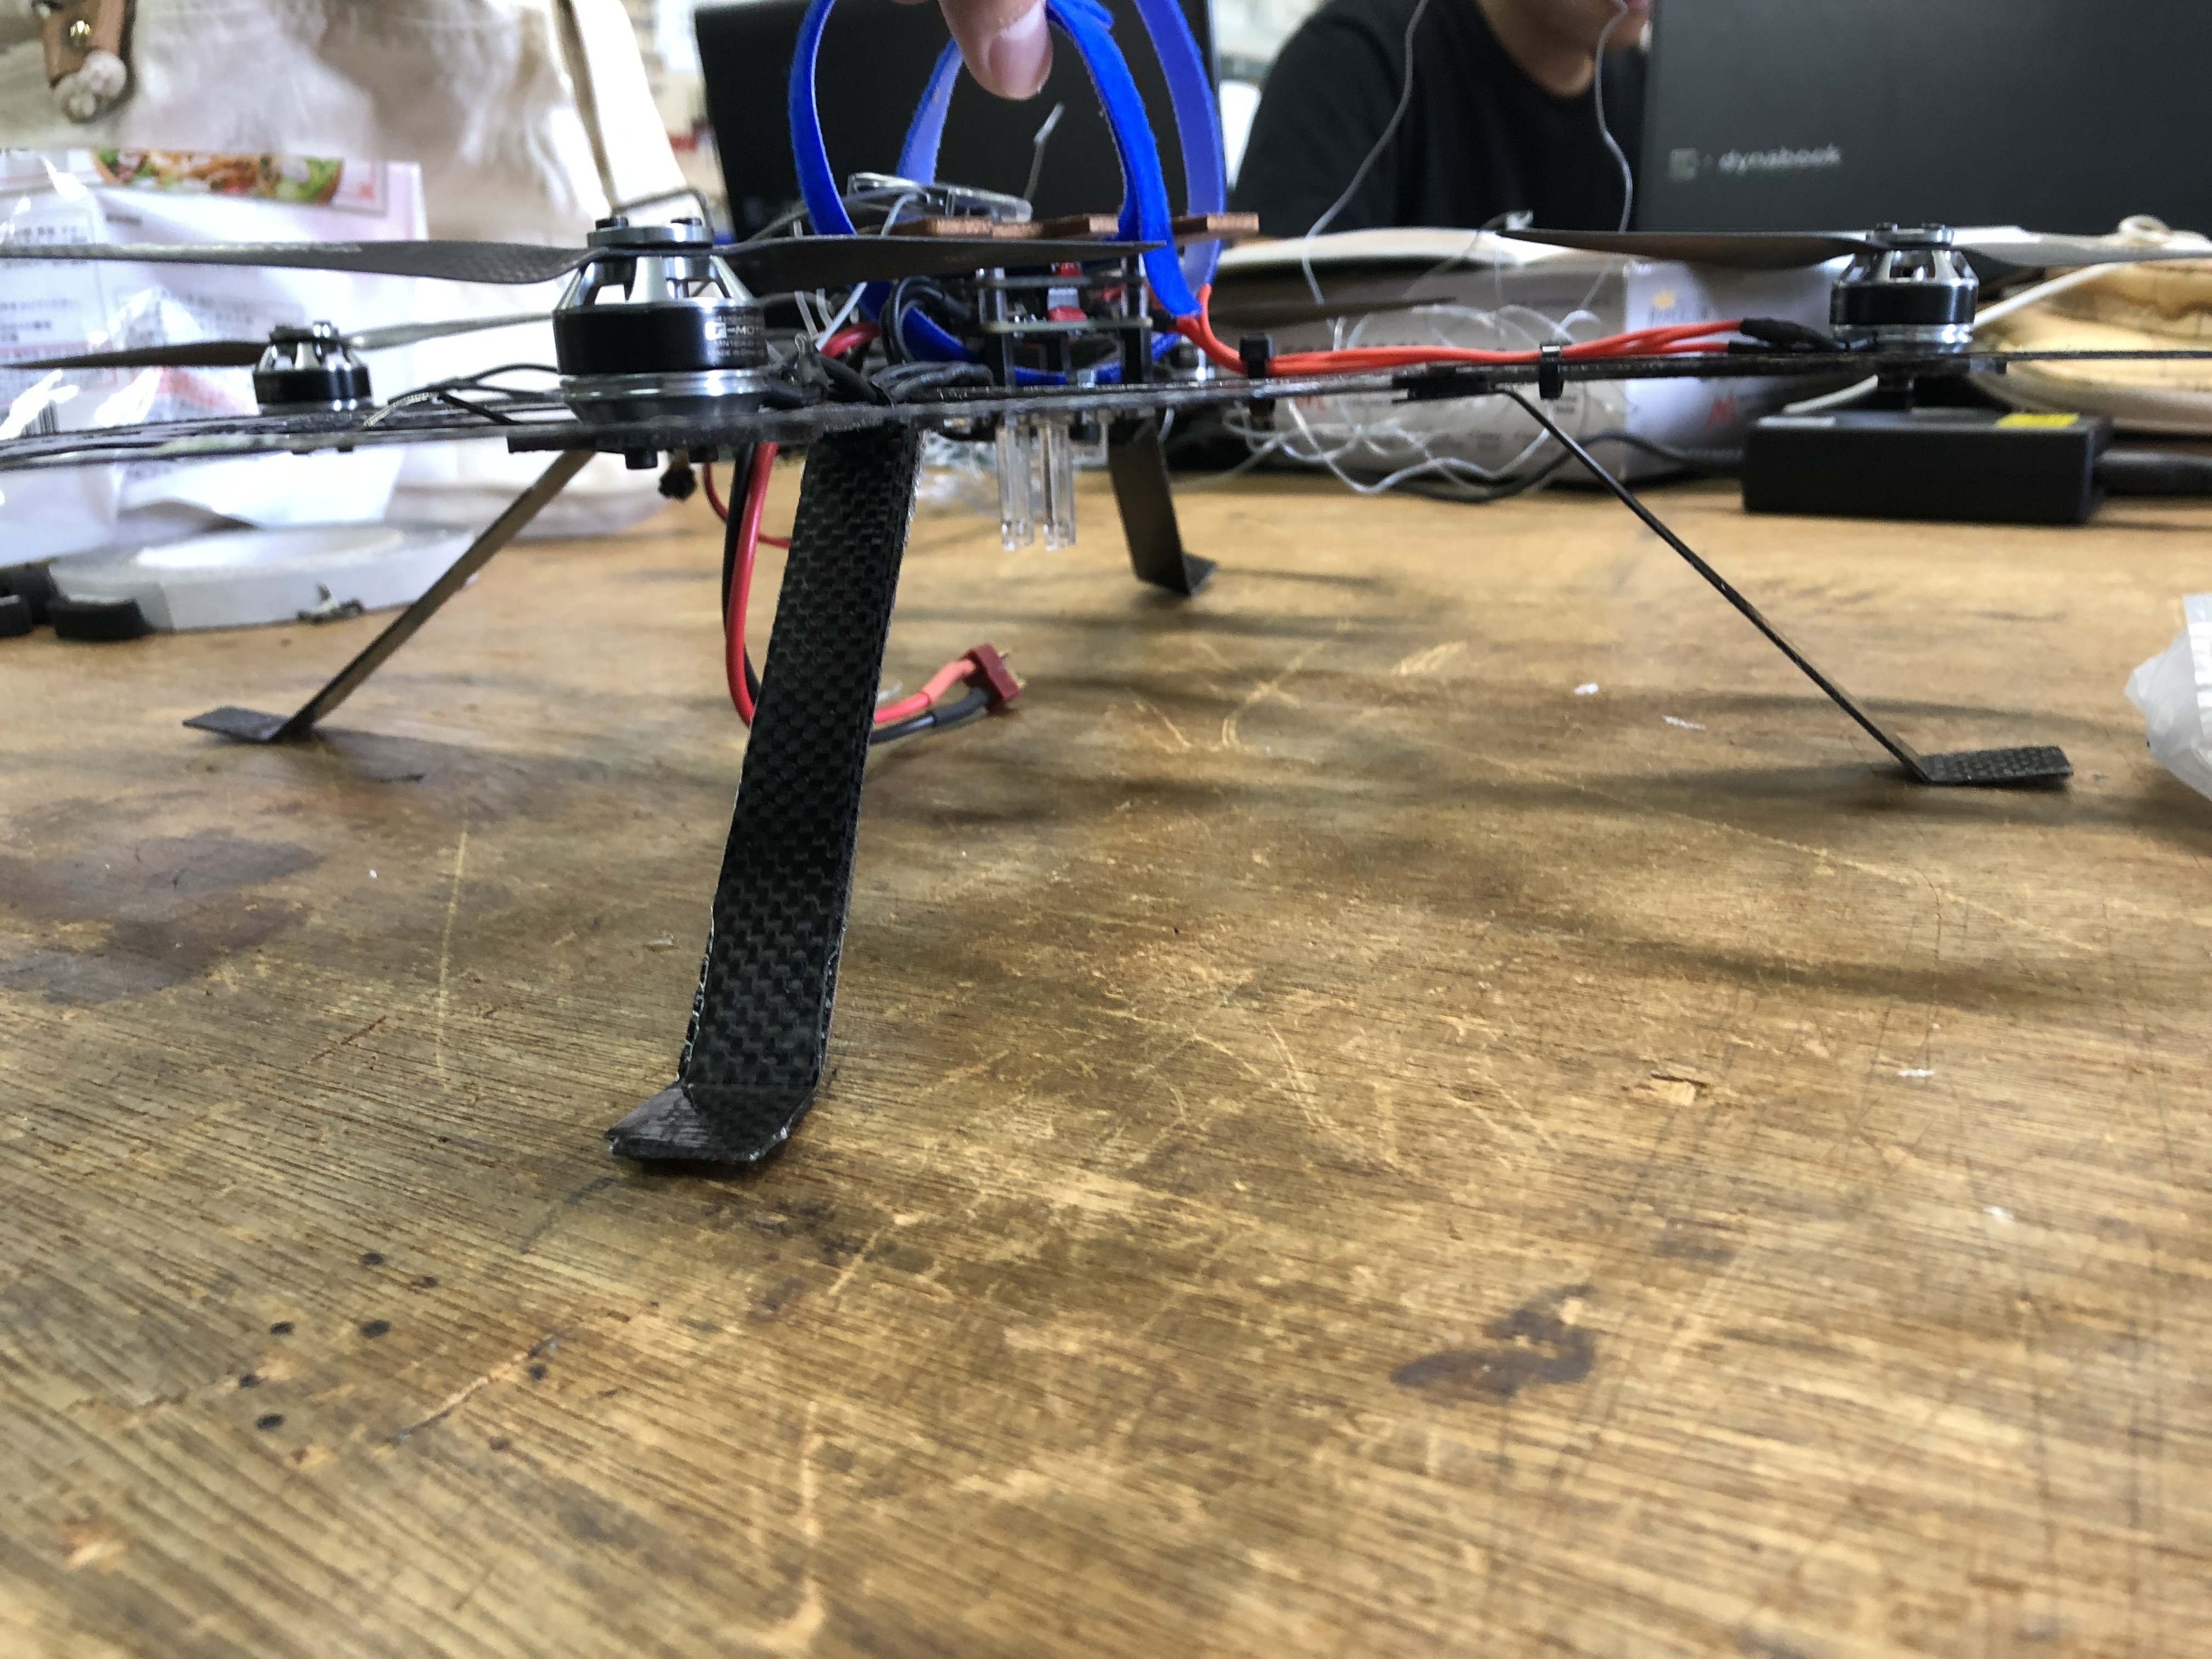
\includegraphics[width=120mm]{img/24.JPG}
    \end{center}
  \caption{平面積層で製作した足}
 \label{fig:robot}
\end{figure}


